\documentclass[12pt,a4paper]{article}

% ─── Page Layout ───────────────────────────────────────────────────────────────
\usepackage[a4paper, margin=0.8in, headheight=14pt]{geometry}

% ─── Fonts (XeLaTeX) ───────────────────────────────────────────────────────────
\usepackage{fontspec}
\usepackage{unicode-math}
\setmainfont{TeX Gyre Pagella}
\setmonofont[Scale=0.88]{TeX Gyre Cursor}
\setmathfont{Latin Modern Math}

% ─── Packages ──────────────────────────────────────────────────────────────────
\usepackage{xcolor}
\usepackage{colortbl}
\usepackage{titlesec}
\usepackage{enumitem}
\usepackage{tabularx}
\usepackage{booktabs}
\usepackage{array}
\usepackage{amsmath}
\usepackage{tikz}
\usetikzlibrary{shapes.geometric, arrows.meta, positioning, calc, fit, decorations.pathreplacing, patterns}
\usepackage[american]{circuitikz}
\usepackage{tcolorbox}
\tcbuselibrary{skins, breakable}
\usepackage{hyperref}
\usepackage{fancyhdr}
\usepackage{graphicx}
\usepackage{microtype}
\hyphenpenalty=10000
\exhyphenpenalty=10000
\sloppy
\usepackage{caption}
\usepackage{setspace}
\usepackage{multirow}
\usepackage{tocloft}

% ─── Q&A helper ────────────────────────────────────────────────────────────────
\newcommand{\Q}[1]{\textbf{#1}\par\noindent\ignorespaces}

% ─── Colour Palette ────────────────────────────────────────────────────────────
\definecolor{myred}{RGB}{196,30,58}
\definecolor{mydark}{RGB}{30,30,50}
\definecolor{mygreen}{RGB}{14,120,80}
\definecolor{myteal}{RGB}{0,130,140}
\definecolor{myamber}{RGB}{180,100,0}
\definecolor{mypurple}{RGB}{100,30,160}
\definecolor{mygray}{RGB}{246,247,249}
\definecolor{mgframe}{RGB}{180,185,200}
\definecolor{watermark}{RGB}{145,150,170}
\definecolor{hdrred}{RGB}{250,232,235}
\definecolor{hdrgreen}{RGB}{220,244,233}
\definecolor{hdrteal}{RGB}{220,242,244}
\definecolor{hdramber}{RGB}{253,242,215}
\definecolor{hdrpurple}{RGB}{238,228,255}
\definecolor{hdrgray}{RGB}{238,240,245}
\definecolor{rowalt}{RGB}{250,251,253}

% ─── Section Formatting ────────────────────────────────────────────────────────
\titleformat{\section}{\large\bfseries\color{myred}}{\thesection.}{0.5em}{}[\vspace{1pt}{\color{myred}\rule{\linewidth}{0.8pt}}]
\titleformat{\subsection}{\normalsize\bfseries\color{myteal}}{\thesubsection}{0.5em}{}
\titlespacing*{\section}{0pt}{18pt}{7pt}
\titlespacing*{\subsection}{0pt}{11pt}{4pt}

% ─── Paragraph ─────────────────────────────────────────────────────────────────
\setlength{\parindent}{0pt}
\setlength{\parskip}{4pt}

% ─── TOC Styling ───────────────────────────────────────────────────────────────
\renewcommand{\cfttoctitlefont}{\large\bfseries\color{myred}}
\renewcommand{\cftaftertoctitle}{\par\noindent{\color{myred}\rule{\linewidth}{0.8pt}}}
\setlength{\cftbeforetoctitleskip}{0pt}
\setlength{\cftaftertoctitleskip}{6pt}
\renewcommand{\cftsecfont}{\normalsize\bfseries\color{mydark}}
\renewcommand{\cftsecpagefont}{\normalsize\bfseries\color{mydark}}
\renewcommand{\cftsecleader}{\cftdotfill{\cftdotsep}}
\setlength{\cftbeforesecskip}{7pt}
\renewcommand{\cftsubsecfont}{\small\color{mydark}}
\renewcommand{\cftsubsecpagefont}{\small\color{mydark}}
\setlength{\cftbeforesubsecskip}{3pt}
\setlength{\cftsubsecindent}{1.4em}

% ─── Table helpers ─────────────────────────────────────────────────────────────
\renewcommand{\arraystretch}{1.45}
\setlength{\tabcolsep}{6pt}
\arrayrulecolor{mydark}
\newcolumntype{B}[1]{>{\small\bfseries\raggedright\arraybackslash}m{#1}}
\newcolumntype{Y}{>{\small\raggedright\arraybackslash}X}
\renewcommand{\tabularxcolumn}[1]{m{#1}}

% ─── Header / Footer ───────────────────────────────────────────────────────────
\pagestyle{fancy}
\fancyhf{}
\fancyhead[L]{\small\color{myred}\textbf{PE-EC802A}\;\color{mydark}--- Mixed Signal Design}
\fancyhead[R]{\small\color{myteal}\textbf{Module 4 Notes}}
\fancyfoot[C]{\small\color{mydark}\thepage}
\fancyfoot[R]{\small\color{watermark}\textit{\copyright\ Biraj}}
\renewcommand{\headrulewidth}{0.5pt}
\renewcommand{\footrulewidth}{0.3pt}

% ─── Hyperref ──────────────────────────────────────────────────────────────────
\hypersetup{colorlinks=true, linkcolor=myteal, urlcolor=myteal,
  pdfauthor={Biraj Sarkar}, pdftitle={PE-EC802A --- Module 4 Notes}}

% ─── tcolorbox styles ──────────────────────────────────────────────────────────
\tcbset{
  tikzbox/.style={colback=mygray, colframe=mgframe, boxrule=0.6pt, arc=4pt,
    left=8pt, right=8pt, top=6pt, bottom=6pt,
    colbacktitle=mgframe, coltitle=mydark, fonttitle=\small\bfseries},
  defbox/.style={colback=hdrgreen, colframe=mygreen, boxrule=0.8pt, arc=4pt,
    left=9pt, right=9pt, top=6pt, bottom=6pt,
    colbacktitle=mygreen, coltitle=white, fonttitle=\small\bfseries},
  formulabox/.style={colback=hdrteal, colframe=myteal, boxrule=0.8pt, arc=4pt,
    left=9pt, right=9pt, top=7pt, bottom=7pt,
    colbacktitle=myteal, coltitle=white, fonttitle=\small\bfseries},
  examplebox/.style={colback=hdramber, colframe=myamber, boxrule=0.8pt, arc=4pt,
    left=9pt, right=9pt, top=6pt, bottom=6pt,
    colbacktitle=myamber, coltitle=white, fonttitle=\small\bfseries},
  masonbox/.style={colback=hdrpurple, colframe=mypurple, boxrule=0.8pt, arc=4pt,
    left=9pt, right=9pt, top=6pt, bottom=6pt,
    colbacktitle=mypurple, coltitle=white, fonttitle=\small\bfseries},
  exambox/.style={colback=hdrpurple, colframe=mypurple, boxrule=1pt, arc=5pt,
    left=10pt, right=10pt, top=8pt, bottom=8pt,
    colbacktitle=mypurple, coltitle=white, fonttitle=\bfseries,
    breakable, title after break={\textbf{Frequently Asked / Viva Questions (contd.)}}}
}
\tcbset{breakable}

% ─── TikZ styles ───────────────────────────────────────────────────────────────
\tikzset{
  block/.style={rectangle, draw=myteal, fill=hdrteal,
    text width=2.4cm, align=center, minimum height=0.95cm,
    font=\small, rounded corners=3pt, line width=0.7pt},
  redblock/.style={rectangle, draw=myred, fill=hdrred,
    text width=2.4cm, align=center, minimum height=0.95cm,
    font=\small, rounded corners=3pt, line width=0.7pt},
  sumjunc/.style={circle, draw=myamber, fill=hdramber,
    minimum size=0.62cm, font=\small, line width=0.8pt},
  arrow/.style={-Stealth, thick, color=mydark},
  line/.style={thick, color=mydark}
}

% ═══════════════════════════════════════════════════════════════════════════════
\begin{document}
% ═══════════════════════════════════════════════════════════════════════════════

\begin{center}
  {\LARGE\bfseries\color{myred} PE-EC802A --- Mixed Signal Design}\\[5pt]
  {\normalsize\color{mydark} Semester VIII \quad$\bullet$\quad 3L:0T:0P \quad$\bullet$\quad 3 Credits}\\[3pt]
  {\normalsize\color{myteal}\textbf{Module 4 Exam Notes}}\\[3pt]
  {\small\color{mydark} CGEC \;$|$\; B.Tech ECE (2023--27) \;$|$\; \textit{Biraj Sarkar}}
\end{center}
\vspace{2pt}
\noindent{\color{myred}\rule{\linewidth}{1.5pt}}
\vspace{2pt}

\hypersetup{linkcolor=mydark}
\tableofcontents
\hypersetup{linkcolor=myteal}
\newpage

% ===============================================================================
\section{Mixed-Signal Layout Issues \& Mitigation}
% ===============================================================================

In high-performance mixed-signal integrated circuits, fast-switching digital gates inject noise into the shared silicon substrate and power distribution networks, which severely degrades the resolution of sensitive analog blocks (like ADCs and low-noise amplifiers).

\subsection{1. Substrate Coupling}
Digital circuits consist of logic gates that switch states rapidly, drawing transient currents from the supplies. When the source/drain terminals of digital transistors transition, charge is coupled into the common p-substrate wafer via junction capacitances. This noise propagates through the conductive substrate to sensitive analog devices.

\begin{tcolorbox}[tikzbox, title={Cross-Sectional Model of Substrate Noise Coupling and Guard Ring Protection}]
\centering
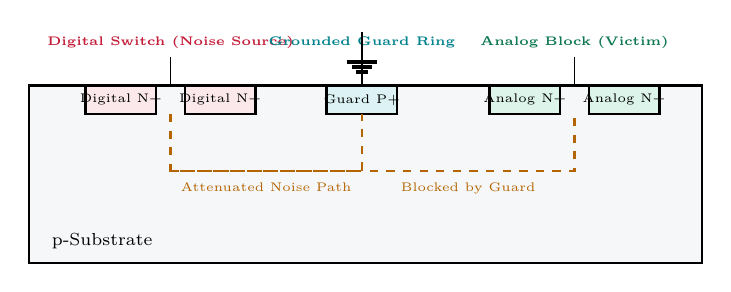
\begin{tikzpicture}[scale=0.9, transform shape]
  % Wafer substrate
  \draw[thick, fill=mygray] (0, 0) rectangle (9.5, -2.5);
  \node[right, font=\scriptsize] at (0.2, -2.2) {p-Substrate};
  
  % Digital noise source (N+ regions)
  \draw[thick, fill=hdrred] (0.8, 0) rectangle (1.8, -0.4);
  \node[font=\tiny] at (1.3, -0.2) {Digital N+};
  \draw[thick, fill=hdrred] (2.2, 0) rectangle (3.2, -0.4);
  \node[font=\tiny] at (2.7, -0.2) {Digital N+};
  \node[above, font=\tiny\bfseries\color{myred}] at (2.0, 0.4) {Digital Switch (Noise Source)};
  \draw (2.0, 0.4) -- (2.0, 0);

  % Guard Ring (P+ region)
  \draw[thick, fill=hdrteal] (4.2, 0) rectangle (5.2, -0.4);
  \node[font=\tiny] at (4.7, -0.2) {Guard P+};
  \node[above, font=\tiny\bfseries\color{myteal}] at (4.7, 0.4) {Grounded Guard Ring};
  \draw[thick] (4.7, 0) -- (4.7, 0.75) node[ground] {};

  % Analog noise victim (N+ regions)
  \draw[thick, fill=hdrgreen] (6.5, 0) rectangle (7.5, -0.4);
  \node[font=\tiny] at (7.0, -0.2) {Analog N+};
  \draw[thick, fill=hdrgreen] (7.9, 0) rectangle (8.9, -0.4);
  \node[font=\tiny] at (8.4, -0.2) {Analog N+};
  \node[above, font=\tiny\bfseries\color{mygreen}] at (7.7, 0.4) {Analog Block (Victim)};
  \draw (7.7, 0.4) -- (7.7, 0);

  % Substrate resistance network (noise paths)
  \draw[thick, dashed, color=myamber] (2.0, -0.4) -- (2.0, -1.2) -- (4.7, -1.2);
  \draw[thick, dashed, color=myamber] (4.7, -1.2) -- (4.7, -0.4);
  \draw[thick, dashed, color=myamber] (2.0, -1.2) -- (7.7, -1.2) -- (7.7, -0.4);
  
  \node[below, font=\tiny\color{myamber}] at (3.35, -1.25) {Attenuated Noise Path};
  \node[below, font=\tiny\color{myamber}] at (6.2, -1.25) {Blocked by Guard};
\end{tikzpicture}
\end{tcolorbox}

\textbf{Mitigation Strategy (Guard Rings):}
A guard ring is a low-impedance ring of diffusion surrounding the circuit blocks.
\begin{itemize}[leftmargin=*, itemsep=2.5pt]
  \item \textbf{p+ Guard Ring:} Implemented in p-substrate, connected to a dedicated quiet analog ground ($V_{SSA}$). It collects hole currents flowing through the substrate from digital noise sources, shunting them to ground before they reach the analog block.
  \item \textbf{n+ Guard Ring in N-well:} Connected to quiet supply ($V_{DDA}$), collecting electron currents and isolating regions.
\end{itemize}

\subsection{2. Power Supply Noise and Ground Bounce}
Power and ground pads on an IC package exhibit parasitic inductance ($L$) and resistance ($R$). When digital gates switch simultaneously, they draw sharp current spikes ($di/dt$), causing a voltage fluctuation on the supply rails:
\[
V_{bounce} = L \frac{di}{dt}
\]
This fluctuation directly modulates the threshold voltages and bias conditions of analog circuits connected to the same supply rails.

\textbf{Mitigation:}
\begin{itemize}[leftmargin=*, itemsep=2pt]
  \item \textbf{Split Supplies:} Separate supply pins and routing traces for analog ($V_{DDA}, V_{SSA}$) and digital ($V_{DDD}, V_{SSD}$) domains.
  \item \textbf{On-Chip Decoupling Capacitors (Decaps):} Placed near supply rails to act as local charge reservoirs, damping high-frequency voltage ripples.
\end{itemize}

% ===============================================================================
\section{Device Matching and Precision Layout}
% ===============================================================================

Matching of on-chip components (capacitors and transistors) is critical for accuracy in data converters and differential amplifiers.

\subsection{1. Types of Mismatch}
Mismatch is categorized as systematic or random.
\begin{itemize}[leftmargin=*, itemsep=2.5pt]
  \item \textbf{Systematic Mismatch:} Caused by deterministic spatial gradients across the wafer (e.g., temperature variations, oxide thickness gradients, lithography light scattering).
  \item \textbf{Random Mismatch:} Caused by microscopic statistical variations (e.g., edge roughness, dopant atom fluctuations).
\end{itemize}

\subsection{2. Common-Centroid Matching for Capacitors}
To cancel the effects of linear spatial gradients (such as oxide thickness variations across a wafer), matching devices must be arranged symmetrically about a common central point (common-centroid configuration).

Consider matching two equal capacitors $C_A$ and $C_B$. If they are placed side-by-side ($A$ next to $B$), a linear gradient in oxide thickness will cause one to be larger than the other. If we split each capacitor into two halves ($A_1, A_2$ and $B_1, B_2$) and arrange them in a one-dimensional or two-dimensional array, the gradient effects cancel.

\begin{tcolorbox}[tikzbox, title={Common-Centroid Capacitor Array Layout (ABBA)}]
\centering
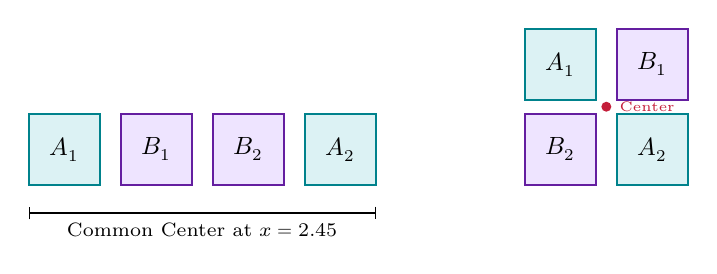
\begin{tikzpicture}[scale=0.9]
  % 1D Common Centroid: A B B A
  \draw[thick, fill=hdrteal, draw=myteal] (0,0) rectangle (1,1) node[pos=0.5, font=\small\bfseries] {$A_1$};
  \draw[thick, fill=hdrpurple, draw=mypurple] (1.3,0) rectangle (2.3,1) node[pos=0.5, font=\small\bfseries] {$B_1$};
  \draw[thick, fill=hdrpurple, draw=mypurple] (2.6,0) rectangle (3.6,1) node[pos=0.5, font=\small\bfseries] {$B_2$};
  \draw[thick, fill=hdrteal, draw=myteal] (3.9,0) rectangle (4.9,1) node[pos=0.5, font=\small\bfseries] {$A_2$};
  
  \draw[|-|] (0,-0.4) -- (4.9,-0.4) node[midway, below, font=\scriptsize] {Common Center at $x = 2.45$};
  
  % 2D Common Centroid Box: 
  % A B
  % B A
  \begin{scope}[xshift=7cm]
    \draw[thick, fill=hdrteal, draw=myteal] (0,1.2) rectangle (1,2.2) node[pos=0.5, font=\small\bfseries] {$A_1$};
    \draw[thick, fill=hdrpurple, draw=mypurple] (1.3,1.2) rectangle (2.3,2.2) node[pos=0.5, font=\small\bfseries] {$B_1$};
    \draw[thick, fill=hdrpurple, draw=mypurple] (0,0) rectangle (1,1) node[pos=0.5, font=\small\bfseries] {$B_2$};
    \draw[thick, fill=hdrteal, draw=myteal] (1.3,0) rectangle (2.3,1) node[pos=0.5, font=\small\bfseries] {$A_2$};
    
    \fill[myred] (1.15, 1.1) circle (2pt);
    \node[right, font=\tiny\color{myred}] at (1.2, 1.1) {Center};
  \end{scope}
\end{tikzpicture}
\end{tcolorbox}

By connecting $A = A_1 + A_2$ and $B = B_1 + B_2$, any linear variation in the horizontal or vertical direction affects both groups equally, preserving the ratio $C_A/C_B = 1$.

% ===============================================================================
\section{Low-Voltage Differential Signaling (LVDS)}
% ===============================================================================

\subsection{Single-Ended vs. Differential Signaling}
Single-ended signaling routes signals as a voltage relative to a common ground rail. Any ground bounce or external electromagnetic coupling adds directly to the signal, corrupting it.

Differential signaling uses two complementary lines ($V_p$ and $V_n$) to transmit information. The receiver detects only the difference $V_{diff} = V_p - V_n$.
\begin{itemize}[leftmargin=*, itemsep=2.5pt]
  \item \textbf{Common-Mode Rejection:} Any noise coupled onto the board affects both lines equally. Since the receiver processes only the difference, this common-mode noise is rejected.
  \item \textbf{Reduced EMI:} The magnetic fields generated by the current in the two tightly-coupled differential traces are equal and opposite, cancelling out, which minimizes electromagnetic interference (EMI).
\end{itemize}

\subsection{LVDS Transceiver Interface}
LVDS is a high-speed, low-power physical layer interface standard. It operates by routing a constant current through a differential pair terminated by a resistor.

\begin{tcolorbox}[tikzbox, title={LVDS Transceiver Interface Schematic}]
\centering
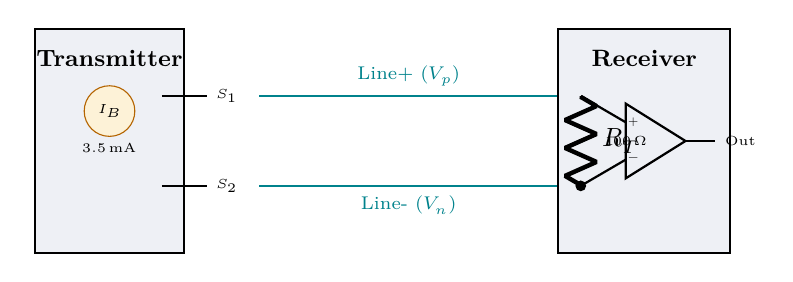
\begin{tikzpicture}[scale=0.95, transform shape]
  % Transmitter box
  \draw[thick, fill=hdrgray] (-2.5, 1.5) rectangle (-0.5, -1.5);
  \node[font=\small\bfseries] at (-1.5, 1.1) {Transmitter};
  \node[draw=myamber, fill=hdramber, circle, minimum size=0.5cm, font=\tiny] (ib) at (-1.5, 0.4) {$I_B$};
  \node[below, font=\tiny] at (-1.5, 0.1) {$3.5\,$mA};
  
  % Switches
  \draw[thick] (-0.8, 0.6) -- (-0.2, 0.6) node[right, font=\tiny] {$S_1$};
  \draw[thick] (-0.8, -0.6) -- (-0.2, -0.6) node[right, font=\tiny] {$S_2$};
  
  % Transmission Lines
  \draw[thick, color=myteal] (0.5, 0.6) -- (4.5, 0.6) node[midway, above, font=\scriptsize] {Line+ ($V_p$)};
  \draw[thick, color=myteal] (0.5, -0.6) -- (4.5, -0.6) node[midway, below, font=\scriptsize] {Line- ($V_n$)};
  
  % Receiver
  \draw[thick, fill=hdrgray] (4.5, 1.5) rectangle (6.8, -1.5);
  \node[font=\small\bfseries] at (5.65, 1.1) {Receiver};
  
  % Termination resistor
  \draw[thick] (4.8, 0.6) to[R, l=$R_T$, -*] (4.8, -0.6);
  \node[right, font=\tiny] at (5.0, 0.0) {$100\,\Omega$};
  
  % Differential Receiver Op-amp
  \draw[thick] (5.4, 0.5) -- (5.4, -0.5) -- (6.2, 0.0) -- cycle;
  \node[font=\tiny] at (5.5, 0.25) {$+$};
  \node[font=\tiny] at (5.5, -0.25) {$-$};
  \draw[thick] (4.8, 0.6) -- (5.4, 0.25);
  \draw[thick] (4.8, -0.6) -- (5.4, -0.25);
  \draw[thick] (6.2, 0.0) -- (6.6, 0.0) node[right, font=\tiny] {Out};
\end{tikzpicture}
\end{tcolorbox}

\textbf{Key Parameters:}
\begin{enumerate}[label=\textbf{\arabic*.}, leftmargin=*, itemsep=3.5pt]
  \item \textbf{Current Loop:} The transmitter contains a $3.5\,$mA current source. Depending on the digital state, the switches route this current down either $V_p$ or $V_n$.
  \item \textbf{Termination:} The current flows through the transmission line and passes through the $100\,\Omega$ termination resistor $R_T$ at the receiver, then returns via the other line.
  \item \textbf{Voltage Swing:} The voltage swing across $R_T$ is:
  \[
  V_{diff} = I_{loop} \times R_T = 3.5\,\text{mA} \times 100\,\Omega = 350\,\text{mV}
  \]
  This small voltage swing allows extremely fast switching and minimizes power consumption.
  \item \textbf{Common-Mode Voltage:} The nominal common-mode voltage is set to $1.2\,$V, which is compatible with low-voltage supply rails.
\end{enumerate}

% ===============================================================================
% QUICK REVISION PAGE
% ===============================================================================
\newpage
\begin{center}
  {\large\bfseries\color{myred} Quick Revision --- Module 4}\\[3pt]
  {\small\color{mydark} Layout \& Signaling $|$ PE-EC802A}
\end{center}
\noindent{\color{myred}\rule{\linewidth}{1.2pt}}
\vspace{4pt}

\begin{tcolorbox}[formulabox, title={\textbf{Key Formulas at a Glance}}]
\renewcommand{\arraystretch}{1.35}
\begin{tabularx}{\linewidth}{B{5.0cm} X}
Ground Bounce Voltage & $V_{bounce} = L \frac{di}{dt}$ \\[4pt]
LVDS Current Loop & $I_{loop} = 3.5\,$mA \\[4pt]
LVDS Differential Swing & $V_{diff} = I_{loop} \times R_T = 350\,$mV \\[4pt]
LVDS Termination Resistor & $R_T = 100\,\Omega$ \\[4pt]
LVDS Common-Mode Voltage & $V_{CM} = 1.2\,$V \\[4pt]
\end{tabularx}
\end{tcolorbox}

\begin{tcolorbox}[defbox, title={\textbf{One-Line Definitions}}]
\begin{itemize}[leftmargin=*, itemsep=2pt, topsep=0pt]
  \item \textbf{Substrate Coupling:} Injection of digital switching noise into the shared silicon substrate, victimizing analog nodes.
  \item \textbf{Guard Ring:} A low-resistance diffusion ring surrounding sensitive analog components to collect substrate noise currents.
  \item \textbf{Ground Bounce:} Inductive supply noise caused by high $di/dt$ transitions across package lead inductances.
  \item \textbf{Systematic Mismatch:} Mismatch on silicon caused by deterministic spatial gradients across the wafer.
  \item \textbf{Random Mismatch:} Mismatch on silicon caused by microscopic statistical variations (e.g., dopant fluctuations).
  \item \textbf{Common-Centroid Layout:} Symmetrical layout arrangement of matched devices around a single central point to cancel linear gradients.
  \item \textbf{LVDS:} A high-speed differential signaling standard that transmits data using a $3.5\,$mA current loop over $100\,\Omega$.
\end{itemize}
\end{tcolorbox}

\begin{tcolorbox}[exambox, title={\textbf{Frequently Asked / Viva Questions}}]
\begin{enumerate}[topsep=0pt, label=\textbf{Q\arabic*.}, itemsep=5pt]
  \item \Q{How does substrate coupling occur in mixed-signal ICs?}
    When digital circuits switch states, transient currents flow through junction capacitances into the shared p-type substrate. These currents travel through the silicon wafer and couple into the bodies of sensitive analog transistors, shifting their thresholds.
  \item \Q{What is a guard ring, and how does it protect analog circuitry?}
    A guard ring is a ring of p+ diffusion (grounded) or n+ diffusion (connected to $V_{DD}$) surrounding a circuit. It collects substrate noise currents and shunts them to a quiet power supply before they can reach sensitive analog blocks.
  \item \Q{Explain the physical mechanism behind ground bounce.}
    Ground bounce is caused by the parasitic inductance of package wires/pads. When multiple digital outputs switch states simultaneously, they draw high transient currents ($di/dt$). The inductive voltage drop ($V = L di/dt$) causes the ground potential to bounce.
  \item \Q{How do split supply domains help in mixed-signal chips?}
    By separating the supply pads and lines for analog ($V_{DDA}, V_{SSA}$) and digital ($V_{DDD}, V_{SSD}$) domains, ground bounce and digital supply ripple are prevented from directly modulating analog circuit nodes.
  \item \Q{What is the purpose of common-centroid layout in capacitor matching?}
    It arranges split capacitor cells symmetrically around a central point. Any linear spatial variation in oxide thickness or temperature affects both matching groups equally, cancelling the ratio error.
  \item \Q{What is the difference between systematic and random device mismatch?}
    Systematic mismatch is caused by deterministic spatial gradients (like temperature or process variations) and can be minimized by layout techniques. Random mismatch is caused by random statistical variations (like dopant fluctuations) and can only be reduced by scaling up device dimensions.
  \item \Q{Explain the working principle of LVDS signaling.}
    LVDS uses a constant current source ($3.5\,$mA) at the transmitter. The digital state controls switches to route this current through a differential trace pair. A $100\,\Omega$ resistor at the receiver terminates the lines, converting the current into a $350\,$mV voltage swing.
  \item \Q{Why does differential signaling provide high noise immunity?}
    External noise couples equally onto both differential traces (common-mode noise). Since the receiver detects only the difference between the two lines, this common-mode noise is rejected.
  \item \Q{State the nominal parameters of an LVDS interface.}
    Loop current: $3.5\,$mA; Termination resistance: $100\,\Omega$; Differential swing: $350\,$mV; Common-mode voltage: $1.2\,$V.
  \item \Q{Why does LVDS generate very low Electromagnetic Interference (EMI)?}
    The currents in the differential pair are equal and opposite, flowing in close proximity. The magnetic fields they generate cancel each other out, minimizing electromagnetic radiation.
\end{enumerate}
\end{tcolorbox}

\end{document}
